\subsubsection{Module 4: Hệ thống Quản trị (Admin System)}
Module này cung cấp các công cụ quyền lực cho Quản trị viên (Admin) để giám sát người dùng, kiểm duyệt nội dung và theo dõi sức khỏe của toàn bộ hệ thống.

\begin{figure}[H]
\centering
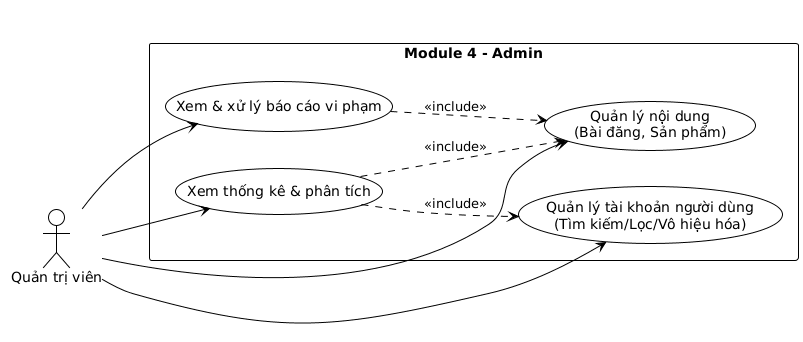
\includegraphics[width=\textwidth]{Images/Usecases/UC-M4-Admin.png}
\caption{Sơ đồ Use Case cho Module 4: Hệ thống Quản trị}
\label{fig:usecase-module4}
\end{figure}

\renewcommand{\arraystretch}{1.3}

% =====================================================
% UC4.1: QUẢN LÝ TÀI KHOẢN NGƯỜI DÙNG
% =====================================================
\begin{table}[H]
\centering
\begin{tabularx}{\textwidth}{|l|X|}
\hline
\textbf{Tên Use Case} & \textbf{UC4.1: Quản lý tài khoản người dùng} \\ \hline
\textbf{Tác nhân} & Quản trị viên (Admin) \\ \hline
\textbf{Mô tả} & Cung cấp cho quản trị viên các công cụ để xem, tìm kiếm, lọc và thực hiện các hành động trên tài khoản người dùng như vô hiệu hóa hoặc cấp lại quyền. \\ \hline
\textbf{Kích hoạt} & Quản trị viên truy cập vào mục ``Quản lý Người dùng'' trong Bảng điều khiển quản trị (Admin Dashboard). \\ \hline
\textbf{Điều kiện tiên quyết} & Quản trị viên đã đăng nhập vào hệ thống với quyền hạn phù hợp. \\ \hline
\textbf{Điều kiện sau} & Thông tin hoặc trạng thái của một hoặc nhiều tài khoản người dùng được thay đổi (ví dụ: tài khoản bị vô hiệu hóa). \\ \hline
\textbf{Luồng sự kiện chính} & 
\begin{enumerate}
    \item Quản trị viên truy cập trang quản lý người dùng.
    \item Hệ thống hiển thị danh sách tất cả người dùng.
    \item Quản trị viên sử dụng các bộ lọc để tìm kiếm người dùng theo tiêu chí.
    \item Quản trị viên chọn một tài khoản người dùng để xem thông tin chi tiết.
    \item Quản trị viên thực hiện một hành động (ví dụ: nhấn nút ``Vô hiệu hóa tài khoản'').
    \item Hệ thống yêu cầu xác nhận hành động.
    \item Quản trị viên xác nhận, và hệ thống cập nhật trạng thái của tài khoản.
\end{enumerate} \\ \hline
\textbf{Ngoại lệ} & 
\begin{itemize}
    \item E1: Quản trị viên cố gắng thực hiện hành động trên tài khoản quản trị viên khác có quyền hạn cao hơn $\rightarrow$ Hệ thống từ chối.
\end{itemize} \\ \hline
\textbf{Ghi chú} & Chức năng này giúp admin duy trì sự kiểm soát đối với cộng đồng người dùng. \\ \hline
\end{tabularx}
\caption{Đặc tả Use Case Quản lý người dùng}
\end{table}

% =====================================================
% UC4.2: QUẢN LÝ NỘI DUNG
% =====================================================
\begin{table}[H]
\centering
\begin{tabularx}{\textwidth}{|l|X|}
\hline
\textbf{Tên Use Case} & \textbf{UC4.2: Quản lý nội dung (Bài đăng/Sản phẩm)} \\ \hline
\textbf{Tác nhân} & Quản trị viên \\ \hline
\textbf{Mô tả} & Cho phép quản trị viên tìm kiếm, xem và xóa các nội dung do người dùng tạo ra như bài đăng hoặc sản phẩm không phù hợp. \\ \hline
\textbf{Kích hoạt} & Quản trị viên truy cập vào các mục quản lý nội dung (ví dụ: ``Quản lý Bài đăng'', ``Quản lý Sản phẩm'') trong dashboard. \\ \hline
\textbf{Điều kiện tiên quyết} & Quản trị viên đã đăng nhập vào hệ thống. \\ \hline
\textbf{Điều kiện sau} & Nội dung không phù hợp (bài đăng, sản phẩm) bị xóa khỏi hệ thống. \\ \hline
\textbf{Luồng sự kiện chính} & 
\begin{enumerate}
    \item Quản trị viên chọn mục nội dung cần quản lý.
    \item Hệ thống hiển thị danh sách các nội dung liên quan.
    \item Quản trị viên sử dụng bộ lọc để tìm kiếm nội dung.
    \item Quản trị viên chọn một nội dung để xem xét.
    \item Nếu nội dung vi phạm, quản trị viên nhấn nút ``Xóa''.
    \item Hệ thống xác nhận và xóa nội dung khỏi cơ sở dữ liệu.
\end{enumerate} \\ \hline
\textbf{Ghi chú} & Việc kiểm duyệt nội dung là cần thiết để giữ cho nền tảng lành mạnh. \\ \hline
\end{tabularx}
\caption{Đặc tả Use Case Quản lý nội dung}
\end{table}

% =====================================================
% UC4.3: XỬ LÝ BÁO CÁO VI PHẠM
% =====================================================
\begin{table}[H]
\centering
\begin{tabularx}{\textwidth}{|l|X|}
\hline
\textbf{Tên Use Case} & \textbf{UC4.3: Xem và xử lý báo cáo vi phạm} \\ \hline
\textbf{Tác nhân} & Quản trị viên \\ \hline
\textbf{Mô tả} & Cho phép quản trị viên xem lại các báo cáo vi phạm được gửi bởi người dùng và đưa ra hành động xử lý phù hợp (ví dụ: xóa nội dung, khóa tài khoản). \\ \hline
\textbf{Điều kiện tiên quyết} & 
\begin{itemize}
    \item Quản trị viên đã đăng nhập vào hệ thống.
    \item Có ít nhất một báo cáo từ người dùng được gửi đến hệ thống.
\end{itemize} \\ \hline
\textbf{Điều kiện sau} & 
\begin{itemize}
    \item Báo cáo được đánh dấu là ``đã xử lý''.
    \item Hành động xử lý đối với nội dung hoặc người dùng bị báo cáo được thực thi.
\end{itemize} \\ \hline
\textbf{Luồng sự kiện chính} & 
\begin{enumerate}
    \item Quản trị viên vào trang quản lý báo cáo.
    \item Hệ thống hiển thị danh sách các báo cáo chưa được xử lý, sắp xếp theo mức độ ưu tiên.
    \item Quản trị viên chọn một báo cáo để xem chi tiết.
    \item Quản trị viên điều hướng đến nội dung/người dùng bị báo cáo để kiểm tra.
    \item Dựa trên kết quả, quản trị viên quyết định hành động (ví dụ: Xóa bài đăng).
    \item Quản trị viên thực hiện hành động thông qua các công cụ quản lý.
    \item Quản trị viên đánh dấu báo cáo là ``Đã xử lý''.
\end{enumerate} \\ \hline
\textbf{Luồng thay thế} & 
\begin{itemize}
    \item A1: Quản trị viên xác định báo cáo là không hợp lệ và đánh dấu là ``Từ chối''.
\end{itemize} \\ \hline
\textbf{Ngoại lệ} & 
\begin{itemize}
    \item E1: Nội dung bị báo cáo đã được người dùng tự xóa trước khi admin xử lý $\rightarrow$ Admin đánh dấu báo cáo là đã giải quyết.
\end{itemize} \\ \hline
\textbf{Ghi chú} & Đây là chức năng tương tác trực tiếp với phản hồi của cộng đồng để duy trì một môi trường an toàn. \\ \hline
\end{tabularx}
\caption{Đặc tả Use Case Xử lý báo cáo}
\end{table}

% =====================================================
% UC4.4: THỐNG KÊ HỆ THỐNG
% =====================================================
\begin{table}[H]
\centering
\begin{tabularx}{\textwidth}{|l|X|}
\hline
\textbf{Tên Use Case} & \textbf{UC4.4: Xem thống kê và phân tích hệ thống} \\ \hline
\textbf{Tác nhân} & Quản trị viên \\ \hline
\textbf{Mô tả} & Cung cấp các biểu đồ và số liệu thống kê trực quan để quản trị viên theo dõi sự phát triển và ``sức khỏe'' của nền tảng. \\ \hline
\textbf{Kích hoạt} & Quản trị viên truy cập vào mục ``Thống kê \& Phân tích'' trong dashboard. \\ \hline
\textbf{Điều kiện tiên quyết} & Quản trị viên đã đăng nhập vào hệ thống. \\ \hline
\textbf{Điều kiện sau} & Quản trị viên nắm được các chỉ số quan trọng về hoạt động của hệ thống để đưa ra quyết định vận hành. \\ \hline
\textbf{Luồng sự kiện chính} & 
\begin{enumerate}
    \item Quản trị viên truy cập trang thống kê.
    \item Hệ thống truy vấn và tổng hợp dữ liệu.
    \item Hệ thống hiển thị các thông tin tổng quan (tổng số người dùng, sản phẩm, bài đăng).
    \item Hệ thống hiển thị các biểu đồ trực quan, chẳng hạn như: Biểu đồ đường thể hiện số lượng người dùng mới; Biểu đồ tròn thể hiện tỷ lệ giữa người mua và người bán.
    \item Quản trị viên có thể thay đổi khoảng thời gian xem thống kê (ví dụ: 7 ngày qua, 30 ngày qua).
\end{enumerate} \\ \hline
\textbf{Ngoại lệ} & 
\begin{itemize}
    \item E1: Lỗi khi tổng hợp dữ liệu $\rightarrow$ Hệ thống báo lỗi.
\end{itemize} \\ \hline
\textbf{Ghi chú} & Các công cụ phân tích này rất quan trọng để theo dõi sự tăng trưởng của hệ thống. \\ \hline
\end{tabularx}
\caption{Đặc tả Use Case Thống kê hệ thống}
\end{table}